\section{Metode Pengalamatan (Addressing Modes)}

\compiler{Addressing Modes} menentukan bagaimana operan diambil dari memori atau register pada tingkat bahasa mesin. Intermediate Code Generation bertindak sebagai jembatan antara front-end yang dependen pada bahasa sumber dan back-end yang dependen pada mesin target \cite{jhu2024compilers}.

\subsection{Jenis Pengalamatan Umum}
\begin{itemize}
    \item \textbf{Register Addressing}: Operan berada langsung di register (\code{ADD R1, R2}). Sangat cepat karena tidak ada akses memori.
    \item \textbf{Immediate Addressing}: Operan adalah konstanta yang tertanam dalam instruksi (\code{ADDI R1, R1, 10}).
    \item \textbf{Displacement/Indexed}: Mengakses memori dengan alamat \textit{base register} ditambah \textit{offset} (\code{LW R1, 8(R2)}). Sangat berguna untuk \textit{stack frame} dan akses \textit{struct}.
\end{itemize}

\subsection{Complex Addressing Modes (CISC)}
Arsitektur seperti x86 mendukung mode yang lebih kompleks untuk mendukung abstraksi bahasa tingkat tinggi secara langsung di perangkat keras:
\[ \text{Alamat Efektif} = \text{Base} + (\text{Index} \times \text{Scale}) + \text{Displacement} \]
Di mana \textit{Scale} biasanya bernilai 1, 2, 4, atau 8—cocok untuk ukuran data dasar (\texttt{char}, \texttt{short}, \texttt{int}, \texttt{double}).

\subsection{Instruksi LEA (Load Effective Address)}
Instruksi \code{LEA} pada x86 adalah "trik" yang sering digunakan kompilator. Meskipun secara teknis merupakan instruksi pengalamatan, \code{LEA} sebenarnya melakukan kalkulasi aritmatika tanpa mengakses memori.
\begin{itemize}
    \item Contoh: \code{LEA EAX, [EBX + ECX*4]} menghitung $EBX + 4 \times ECX$ dan menyimpan hasilnya di EAX.
    \item Kompilator menggunakan ini untuk perkalian cepat (misal: kali 5, kali 9) dalam satu instruksi.
\end{itemize}

\begin{figure}[!htbp]
    \centering
    \adjustbox{max width=0.8\textwidth,center}{%
    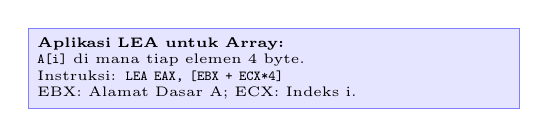
\begin{tikzpicture}[
        rect/.style={rectangle, draw=blue!50, fill=blue!10, text width=6cm, font=\tiny}
    ]
    \node[rect] (lea) {
        \textbf{Aplikasi LEA untuk Array:}\\
        \texttt{A[i]} di mana tiap elemen 4 byte.\\
        Instruksi: \texttt{LEA EAX, [EBX + ECX*4]}\\
        EBX: Alamat Dasar A; ECX: Indeks i.
    };
    \end{tikzpicture}%
    }
    \caption{Efisiensi Pengalamatan Kompleks pada Kompiler}
\end{figure}
